\documentclass[A4paper,oneside,fleqn,11pt]{article}

% This first part of the file is called the PREAMBLE. It includes
% customizations and command definitions. The preamble is everything
% between \documentclass and \begin{document}.

%Cambiamos un poquito los márgenes%
\addtolength{\oddsidemargin}{-1in}
\addtolength{\evensidemargin}{-1in}
\addtolength{\textwidth}{2in}
\addtolength{\topmargin}{-1in}
\addtolength{\textheight}{2in}



\usepackage{mathtools}
\usepackage{graphicx}              % to include figures
\usepackage{amsmath}               % great math stuff
\usepackage{amsmath,scalerel}
\usepackage{amsfonts}              % for blackboard bold, etc
\usepackage{amsthm}                % better theorem environments
\usepackage{amssymb}
\usepackage{mathrsfs}
\usepackage[spanish]{babel}
\usepackage[utf8]{inputenc}
\usepackage{hyperref}
\usepackage{multicol}
\usepackage{tikz-cd}
\usepackage{amsmath}
%\usepackage[linesnumbered,ruled]{algorithm2e}
\usepackage{algpseudocode}
\usetikzlibrary{calc}
\usetikzlibrary{matrix}
\usepackage{graphicx,wrapfig,lipsum}
\usepackage{subcaption} %para poner varias imagenes en un figure
\usepackage{graphicx} % Required for including pictures

\usepackage{sidecap}%para poner la descripción de una imagen al lado de la imagen,no abajo ni arriba
\usepackage{float} % Allows putting an [H] in \begin{figure} to specify the exact location of the figure
\usepackage{wrapfig} % Allows in-line images such as the example fish picture
\graphicspath{ {Grphs/} }


\setcounter{tocdepth}{3}% to get subsubsections in toc

\let\oldtocsection=\tocsection

\let\oldtocsubsection=\tocsubsection

\let\oldtocsubsubsection=\tocsubsubsection

% various theorems, numbered by section

\newtheorem{teo}{Teorema}[section]
\newtheorem{lem}[teo]{Lema}
\newtheorem{prop}[teo]{Proposición}
\newtheorem{cor}[teo]{Corolario}
\newtheorem{crit}[teo]{Criterio}
\newtheorem{propi}[teo]{Propiedad}

\theoremstyle{definition}
\newtheorem{ejcio}[teo]{Ejercicio}
\newtheorem{conj}[teo]{Conjetura}
\newtheorem{obs}[teo]{Observación}
\newtheorem{defn}[teo]{Definición}
\newtheorem{ax}[teo]{Axioma}
\newtheorem{ex}[teo]{Ejemplo}

\newcommand{\bd}[1]{\mathbf{#1}}  % for bolding symbols
\newcommand{\cl}[1]{\overline{#1}} 
\newcommand{\CC}{\mathbb{C}}
\newcommand{\RR}{\mathbb{R}}      % for Real numbers
\newcommand{\ZZ}{\mathbb{Z}}      % for Integers
\newcommand{\NN}{\mathbb{N}}
\newcommand{\QQ}{\mathbb{Q}}
\newcommand{\FF}{\mathbb{F}}
\newcommand{\col}[1]{\left[\begin{matrix} #1 \end{matrix} \right]}
\newcommand{\comb}[2]{\binom{#1^2 + #2^2}{#1+#2}}
\newcommand{\eps}{\varepsilon}
\renewcommand{\hom}{\mathrm{Hom}}
\let\oldemptyset\emptyset
\let\emptyset\varnothing
\DeclareMathOperator{\id}{id}
\DeclareMathOperator{\mcm}{mcm}
\DeclareMathOperator{\mcd}{mcd}
\DeclareMathOperator{\ord}{ord}
\DeclareMathOperator{\im}{im}
\DeclareMathOperator{\End}{End}
\DeclareMathOperator{\Aut}{Aut}
\DeclareMathOperator{\sg}{sg}
\DeclareMathOperator{\cok}{cok}
\DeclareMathOperator{\ext}{Ext}
\DeclareMathOperator{\Obj}{Obj}
\DeclareMathOperator{\rank}{rk}
\DeclareMathOperator{\gr}{gr}
\DeclareMathOperator{\car}{char}
\DeclareMathOperator{\Nil}{Nil}
\DeclareMathOperator{\spec}{Spec}
\DeclareMathOperator{\ev}{ev}
\DeclareMathOperator{\ann}{Ann}
\DeclareMathOperator{\tr}{Tr}
\DeclareMathOperator*{\bigcdot}{\scalerel*{\cdot}{\bigodot}}
\def\acts{\curvearrowright}
\def\stca{\curvearrowleft}

\setcounter{tocdepth}{10}
\setcounter{secnumdepth}{10}

\usepackage[utf8]{inputenc}
\usepackage{fancyhdr}


\begin{document}

%----------------------------------------------------------------------------------------
%	TITLE PAGE
%----------------------------------------------------------------------------------------

\begin{titlepage}

\center % Center everything on the page

\newcommand{\HRule}{\rule{\linewidth}{0.5mm}} % Defines a new command for the horizontal lines, change thickness here

\textsc{\LARGE Universidad de Buenos Aires}\\[1.5cm] % Name of your university/college
\textsc{\Large Facultad de Ciencias Exactas y Naturales}\\[0.5cm] % Major heading such as course name
\textsc{\large Departamento de Computación}\\[0.5cm] % Minor heading such as course title
\textsc{\large Algoritmos y Estructuras de Datos III}\\[0.5cm] % Minor heading such as course title

\HRule \\[0.8cm]
{ \huge \bfseries Trabajo Práctico 3}\\[0.4cm] % Title of your document
\HRule \\[1.5cm]

\begin{minipage}{0.8\textwidth}
\center
%\begin{flushleft} 
\Large
\emph{Autores:}


{Nicolás Chehebar, mail: \textit{nicocheh@hotmail.com}, LU: 308/16 

Matías Duran, mail: \textit{mato\_ fede@live.com.ar}, LU: 400/16 

Lucas Somacal, mail: \textit{lsomacal@gmail.com}, LU: 249/16} % Your name
%\end{flushleft}
~
\end{minipage}\\[4cm]

%\includegraphics{Logo}\\[1cm] % Include a department/university logo - this will require the graphicx package

\vfill % Fill the rest of the page with whitespace

\end{titlepage}

%----------------------------------------------------------------------------------------
%	TABLE OF CONTENTS
%----------------------------------------------------------------------------------------


 %\chead{Algo III, TP2, Chehebar, Duran, Somacal}
 
%\title{Algoritmos y Estructuras de Datos III, TP2}
%\author{Nicolás Chehebar, Matías Duran, Lucas Somacal}
%\date{}



\pagenumbering{roman}
\pagenumbering{arabic}
%\maketitle
\tableofcontents
\clearpage







\section{El Juego}
\subsection{Descripción}
El juego es una generalización del popular 4 en línea \footnote{$https://es.wikipedia.org/wiki/Conecta$\_$4$}. Consiste en una grilla de $M$ filas y $N$ columnas en la cual dos jugadores colocan alternadamente una ficha propia (identificada con rojo las de un jugador y azul las del otro). Las fichas se pueden colocar en cualquier columna de la grilla y una vez elegida la columna, esta determina el movimiento, ya que irá a la fila de ''más abajo'' (la de numeración más baja) que esté desocupada. El objetivo de un jugador será lograr tener un línea recta (diagonal, vertical u horizontal) de $C$ fichas propias. Cuando esto suceda, el jugador ganará el partido. Además, cada jugador dispone de $P$ fichas. En caso de que ambos se queden sin fichas y ninguno haya ganado, la partida finaliza en empate. También se da un empate si la grilla queda llena (y ninguno había ganado). Se trata de una generalización del 4 en línea ya que si tomamos parametros $M=6, N=7, C=4, P=21$ se replicarían las condiciones iniciales del juego.
\subsubsection{Ejemplos}




\section{Jugador Óptimo}

\subsection{El algoritmo}

El algoritmo del jugador del punto 1.a brinda un jugador óptimo. Nos asegura que este jugador hará la estrategia ganadora si hubiera. En caso de que esta no exista, realizará una de empate. Y si tampoco existiera esa, jugará indistintamente sabiendo que perderá. Este análisis se realiza jugada a jugada. Para ejemplificar esto, podría suceder que el oponente tenga la estrategia ganadora y en ese caso nuestro jugador hará cualquier movida indistintamente (pues sabe que perderá), pero si en la próxima jugada el oponente no realiza la correspondiente a su estrategia ganadora y da un nuevo estado del tablero en el que esta vez nuestro jugador tiene estrategia ganadora, nuestro jugador jugará y ganará ya que ahora sí tiene estrategia ganadora.

Para lograr esto, utilizamos una técnica algorítmica similar al Backtracking en el sentido de que exploramos todas las soluciones posibles y nos quedamos con la óptima. Pero esta vez tenemos dos jugadores interviniendo en la situación donde lo que uno busca es todo lo contrario a lo que busca el otro. Podemos decir que un tablero finalizado tiene 3 puntajes posibles, 1 si ganamos nosotros, 0 si es empate, -1 si ganó el otro (podríamos sino generalizarlo para todo tablero y que haya un cuarto valor que sea inválido si aún no hemos calculado el valor de dicho tablero). Así, lo que sabemos es que turno a turno, uno quiere maximizar el puntaje y el otro minimizarlo. Es por esto que dicha técnica algorítmica se llama Minimax. 

De esta manera, igual que en Backtracking tenemos un árbol de ejecución donde cada nodo es un estado del tablero y la raíz es el tablero vacío. Cada nodo (que no sea hoja) tendrá $N$ hijos donde cada uno representará que la próxima jugada fue en alguna de las $N$ columnas. De esta forma, recorremos todos los tableros posibles. Según quién comience, en el primer nivel trataremos de maximizar o minimizar, en el siguiente lo contrario y así sucesivamente. Todos los niveles impares minimizarán si empieza el contrincante y maximizarán si empieza nuestro jugador. El que maximiza le asignará a su nodo un puntaje que será el máximo de los puntajes de todos sus hijos. Análogamente el que minimiza le asignará a su nodo un puntaje que será el mínimo de los puntajes de todos sus hijos.

Así, ejecutando dicho algoritmo la raíz tendrá la información de quién tiene la estrategia ganadora, o que ambos pueden asegurar el empate según quién empiece y haya un 1, 0 o -1. Esta es la idea general del algoritmo, lo veremos más claro en pseudocódigo.

\subsubsection{El Pseudocódigo}
Comenzaremos con el \texttt{main} que es donde se hace el intercambio con el juego en sí. Para ello, primero se le ingresan los parámetros del tablero y las condiciones de juego y luego se desarrolla la partida. Esta termina cuando se lee el mensaje ''ganaste'' ''perdiste'' o ''empataste''. En cada iteración del ciclo (es decir, cada turno) se llama a la función \texttt{minimax} (que se detallará luego y es el algoritmo en sí que resuelve el problema).

Antes del ciclo hay un \texttt{If} que es la ejecución del primer turno si empezamos nosotros a jugar ya que el ciclo comienza con la jugada del otro o la finalización del juego. Esto está determinado por un mensaje que se lee al iniciar el ciclo; si es un número, indica en qué columna jugó el adversario, si es el $string$ ''ganaste'', ''perdiste'' o ''empataste'' termina la ejecución.


\begin{algorithm}
	\texttt{leer} parámetros: \textit{color, oponent\_color, columns, rows, c, p}
    inicializar $tablero$
	\texttt{leer} quién empieza
	\If{empiezo yo}
		{
		$movida$ = \texttt{minimax}($rows$, $columns$, $c$, $p$, $tablero$, \textbf{true}, -1).first
		\texttt{AgregarAtras}($tablero[movida]$, 1)
		resto 1 a $p$
		\texttt{jugar}($movida$)		
		}
    \While{$true$}
    	{
    	\texttt{leer} $mensaje$
        \If{el $mensaje$ es de finalización}
        	{
        	\textbf{break}
            }
        \texttt{AgregarAtras}($tablero$[movida del otro jugador], 2)        	
		resto 1 a $p$
        $movida$ = \texttt{minimax}($rows$, $columns$, $c$, $p$, $tablero$, \textbf{true}, -1).first
        \texttt{AgregarAtras}($tablero[movida]$, 1)
        resto 1 a $p$
    	\texttt{jugar}($movida$)
    	}
    \caption{Main}   
\end{algorithm}

El algoritmo del \texttt{minimax} devuelve una tupla de enteros donde el primero es la columna donde se consigue el mejor valor posible, es decir, la jugada óptima desde el tablero de entrada, y el segundo es el mejor valor que se puede conseguir al hacer esa jugada. Se usaron los valores 1, 0 y -1 para asignar los valores respectivos a ganar, empatar o perder. Además, se usó $\infty$ como número de relleno cuando todavía no se había inicializado.

REVISARRRRRRRRRRRRRRRRRRRRRRRRRRRRRRRRRRRRRRRRRRRRRRRRRRRRRRRRRRRRRRRRRRRRRR

\begin{algorithm}

    \Function{minimax}{\textbf{int} rows, \textbf{int} columns, \textbf{int} c, \textbf{int} p, \textit{matriz}(\textbf{int} \textbf{int}) tablero,  \textbf{bool} maximizo, \textbf{int} ultimajugada}
		\If{\texttt{gane}}
			\State \textbf{return} ($\infty$,1)
		\EndIf
		\If{\texttt{perdi}}
			\State \textbf{return} ($\infty$,-1)
		\EndIf
		\If{empate porque no hay más fichas}
			\State \textbf{return} ($\infty$,0)
		\EndIf
		%\State \textit{vector}(pair(\textbf{int},\textbf{int})) posibles = [(1, $\infty$),..,(\textit{columns}, $\infty$)]
		
		\If{empate porque se llenó el tablero}
		    \State \textbf{return} ($\infty$,0)
		\EndIf
		
		\State recursión llamando al siguiente en el árbol de minimax
		
		\If{Maximizo}
		    \State \textbf{return} (columna del máximo, máximo)
		\Else
		    \State \textbf{return} (columna del máximo, máximo)
		\EndIf
		
    \EndFunction




\end{algorithm}

Las funciones \texttt{gane} y \texttt{perdi} devuelven \textbf{true} si con la jugada se gana la partida o se pierde, respectivamente. Ambas consisten en llamar a la funcion \texttt{ganoJugador} pasándole como jugador al 1 o al 2 respectivamente. Esta función va verificando las distintas condiciones de victoria para el jugador que se le pasó por parámetro (es decir, si con la última jugada se forma $c$ en línea vertical, horizontal o diagonal) hasta que encuentre alguna devoliendo \textbf{true}. Si no encuentra, devuelve \textbf{false}.



\subsection{Poda $\alpha$ - $\beta$}


\subsubsection{Algoritmo}


\subsubsection{Pseudocódigo}
Para la poda se reutilizó el mismo código y se hizo un cambio al hacer la recursión. Para no copiar todo el pseudocódigo, a continuación se lo presenta con la inicialización previa de las variables \textit{posibles, mejorPos, mejorValorMaximizo} y \textit{mejorValorMinimizo}. $posibles$ es un vector de tuplas de enteros donde cada elemento representa una columna del tablero. El primer elemento de la tupla es la columna en sí y el segundo es .... Las otras variables se inicializan con los valores del primer elemento de la primera posición de $posibles$, $-\infty$ y $\infty$ respectivamente.

\begin{algorithm}

    \Function{minimaxPoda}{\textbf{int} rows, \textbf{int} columns, \textbf{int} c, \textbf{int} p, matriz(\textbf{int}, \textbf{int}) tablero,  \textbf{bool} maximizo, \textbf{int} $\alpha$, \textbf{int} $\beta$, \textbf{int} ultimajugada}
    \State vector(pair(\textbf{int},\textbf{int})) $posibles$ = [(1, $\infty$),..,(\textit{columns}, $\infty$)]
    \State \textbf{int} \textit{mejorPos} = $posibles[0]$.first
    \State \textbf{int} \textit{mejorValorMaximizo} = $-\infty$
    \State \textbf{int} \textit{mejorValorMinimizo} = $\infty$
    \For{todos los $posibles$}
    	\State matriz(\textbf{int}, \textbf{int}) $tablero2$ = $tablero$
    	\State actualizar $tablero2$ según quién juega
    	%MEJORAR ESTA LINEAAAAAAAAAA
    	\State $posibles[i]$.second = recursión con $tablero2$, $p-1$ e invirtiendo el valor de verdad de $maximizo$
    	\If{$maximizo$ $\land$ $posibles[i]$.second == $mejorValorMaximizo$}
    		\State actualizo $mejorPos$ y $mejorValorMaximizo$
    	\EndIf
    	\If{$\lnot maximizo$ $\land$ $posibles[i]$.second $< mejorValorMinimizo$}
    		\State actualizo $mejorPos$ y $mejorValorMinimizo$
    	\EndIf
    	\State $\alpha$ = max($\alpha$, mejorValorMaximizo)
    	\State $\beta$ = min($\beta$, mejorValorMinimizo)
    	\If{$\alpha$ $\geq$ $\beta$}
    		\State break
    	\EndIf
    \EndFor
    \If{$maximizo$}
    	\State \textbf{return} ($mejorPos$, $mejorValorMaximizo$)
    \Else
    	\State \textbf{return} ($mejorPos$, $mejorValorMinimizo$)
    \EndIf
    \EndFunction

\end{algorithm}


\subsection{Complejidad}

Veremos que la complejidad es $\mathcal{O}(a^b)$ donde $a=|Columnas Donde Es Posible Jugar|$ y $b = \min{|FichasRestantes|$, $|Casillas Libres En El Tablero|}$ que es en particular acotable por $\mathcal{O}(N\textsuperscript{(N*M)})$ ya que a lo sumo se puede jugar en $N$ columnas (no hay mas en el tablero) y a lo sumo hay $N*M$ casillas libres (o sea, el tablero esta vacío). Cabe aclarar que fichas restantes son la fichas restantes totales (las mias + las suyas). Esto es porque el algoritmo de minimax es como un arbol de Backtracking en el sentido de que checkea todas las posibles sucesiones de jugadas que se pueden dar, considerando tanto lo que yo juego como lo que el juega.

Si bien en total hay  menos de $3\textsuperscript{(N*M)})$ tableros posibles (cada casilla puede estar vacía, o tener una ficha de alguno de los dos jugadores, y acota por arriba pues hay casos que no son posibles, como que haya una ficha encima de una vacía) esto no cuenta la cantidad de posibles partidas que se pueden dar, ya que un mismo tablero podría ser alcanzado de varias formas. Pero a cada paso, cada jugador tiene $N$ opciones de jugada y a lo sumo se juega $N*M$ veces (se llena el tablero) y por ende tenemos $N\textsuperscript{(N*M)}$ estados posibles del tablero. Lo que hace el algoritmo es para cada uno de estos tableros, evaluar si hay o no un ganador y en base a eso establecer un puntaje al tablero que es el que transmite minimax. Este checkeo tiene un costo de $\mathcal{O}(c)$ ya que la función por como la implementamos recibe cual fue la última jugada y sabe que el empate solo se puede dar si no quedan fichas o se lleno el tablero o si esta última jugada logro que algun jugador gane. Checkear las primeras dos condiciones es $\mathcal{O}(1)$ sabiendo la cantidad de fichas que me quedan y de filas y columnas (que es un dato que tenemos guardado). Pero si gano con esa ficha solo hay que verificar las $c$ fichas para todos los sentidos y direcciones (8 en total, 4 direcciones con sus dos sentidos cada una), lo que es $8* \mathcal{O}(c)= \mathcal{O}(c)$. 

Luego dado un tablero, conociendo el valor de minimax de sus hijos, queda tomar o bien maximo o minimo segun corresponda, pero como tiene $N$ hijos a lo sumo (si no es hoja) ya que son las $N$ posibles jugadas inmediatas, esto es $\mathcal{O}(N)$. Esta operación la hacemos para todo nodo, como tambien checkear si hay un ganador. Luego la complejidad total es $|Nodos|*\mathcal{O}(N)*\mathcal{O}(c)$ y hemos visto que $|Nodos|=a^b$ por lo que obtenemos una complejidad $\mathcal{O}(N c a^b)$ lo que es acotable, como hemos visto por $\mathcal{O}(N c N\textsuperscript{(N*M)})=\mathcal{O}(c N\textsuperscript{(N+1)*M})$ pero si recordamos que $c<\min{N,M}$ podemos deducir que la complejidad es menor que $\mathcal{O}(N\textsuperscript{((N+1)*M)+1})$.

En cuanto a la complejidad del algoritmo con poda, no hay modificaciones ya que la misma cota es válida puesto que la única diferencia que tiene la poda es que guarda registro de dos valores ($\alpha$ y $\beta$) y los compara a cada paso, lo que es $\mathcal{O}(1)$ y por ende no afecta la complejidad. Si bien la poda corta varias ramas del arbol de minimax, no podemos asegurar una cota de cuantas ramas cortará y por ende la complejidad teórica seguirá siendo la misma. Sin embargo uno espera que la poda se ejecute y varias ramas del arbol no se checkeen, reduciendo asi el tiempo de ejecución en comparación con el algoritmo sin poda.



\subsection{Experimentación}

\subsubsection{Contexto} 


La experimentación se realizó toda en la misma computadora, cuyo procesador era Intel Atom\texttrademark CPU N2600 @ 1.60GHz, de 36 bits physical, 48 bits virtual, con una memoria RAM de 2048 MB.  Para experimentar, se calculó el tiempo que tardaba el algoritmo sin considerar el tiempo de lectura y escritura ni el tiempo que llevaba armar la matriz (ya que se leía un dato, se escribía la matriz y luego se leía el siguiente). 
El tiempo se medía no como tiempo global sino como tiempo de proceso, calculando la cantidad de ticks del reloj (con el tipo clock\_t de C++) y luego se dividía el delta de ticks sobre CLOCKS\_PER\_SEC. En todos los experimentos el tiempo se mide en segundos. El contexto de experimentación será el mismo a lo largo de todo el trabajo.

\subsubsection{Sin poda}
En principio, para verificar experimentalmente que el jugador era óptimo se jugó en tableros pequeños (en particular, de $2\times2, 3\times3, 2\times3, 3\times2, 2\times4, 4\times2, 3\times4, 4\times3$) con un $c=2, 3, 4$ siempre que cumpla la condición del juego ($c\leq min{N,M}$) contra el jugador random. En todos los casos la cantidad de iteraciones fue de $2*3\textsuperscript{(N*M)}$ por lo que todo tablero posible tenía una probabilidad considerable de ser jugado (notar que la cantidad de juegos posibles es menor que  $N\textsuperscript{(N*M)}$ -de hecho es menor que $3\textsuperscript{(N*M)}$ ya que cada casilla tiene o bien nada o ficha de un jugador o del otro-). Tomamos esta cantidad de repeticiones ya que a cada paso lo que se elige es una de $N$ -o menos si hay columnas llenas- opciones donde jugar y esto se repite hasta que termine el juego -a lo sumo se lena la grilla $N*M$ veces-. Así, tenemos tantas iteraciones como secuencias posibles de jugadas, o sea partidas en general. Como el jugador es random equiprobable, la distribución respecto de qué jugada de las posibles realizar es uniforme y lo multiplicamos por 2 para que sea más probable que salga cualquier partida posible (estamos jugando toda partida posible con una probabilidad considerable). Más aún, es una probabilidad bastante alta ya que se puede notar que solo queremos contar todas las opciones de secuencias de jugadas que puede dar el segundo jugador (en este caso el aleatorio), lo que nos provee una cota menor de la cantidad total de jugadas distintas que se le pueden hacer al jugador optimo, acotandolo por $N\textsuperscript{(N*M/2)}$. 

Estos experimentos se repitieron en dos casos cada uno, cuando comenzaba el \texttt{minimax} y cuando comenzaba el random. Además para fijado el jugador que empieza, se repitió con valores de fichas que fueron $p=N*M/2, N*M/3, N*M/4$ donde el primer valor de $p$ aseguraba que se pueda jugar sin límite de fichas (siempre se podría llegar a llenar el tablero) y los otros dos sí imponían un limite de fichas. Luego de cada experimento, nos fijamos en el archivo \texttt{.log} devuelto por dichas iteraciones y en todos se observó el mismo comportamiento:
\begin{itemize}
\item O bien siempre ganaba (lo que nos indica que había estrategia ganadora para el que empieza). Al invertir la situación (cambiando el jugador que empieza), se daba el ítem 3.
\item O bien siempre ganaba o empataba (lo que nos indicaría que la mejor estrategia para ambos resulta en un empate, pero como el jugador random no siempre juega lo mejor, le daba la posibilidad a nuestro jugador de ganar). Al invertir la situación (cambiando el jugador que empieza) se obtenía este mismo ítem.\textbf{CHEHEBAR: QUÉ CAZZO QUISISTE DECIR CON ESTA ÚLTIMA ORACIÓN}
\item O bien siempre ganaba o empataba o perdía (lo que nos indicaría que el que no empieza tiene estrategia ganadora, pero como el jugador random no siempre juega lo mejor, le daba la posibilidad a veces a nuestro jugador de ganar). Al invertir la situación (cambiando el jugador que empieza), se daba el ítem 1.
\end{itemize}

Como se explicó, estas situaciones, en todos estos tableros, reforzaron fuertemente la idea de que se trataba de un jugador óptimo. Cabe aclarar que se realizó solo con tableros pequeños debido a que, para tableros muy grandes el jugador demoraba demasiado tiempo en decidir que jugar (como se vio en la complejidad teórica exponencial, por lo que crecía brutalmente al crecer el tamaño del tablero y la cantidad de columnas) y por ende resultaba inviable realizar una alta cantidad de iteraciones para recorrer una gran cantidad de tableros posibles lo que nos permita reforzar la idea de optimalidad del jugador. 

Pero en tableros pequeños hemos podido comprobar que en todos los tableros que se dieron, cumplieron que el jugador era óptimo ya que si tenía la posibilidad de ganar lo hacía, en caso de que esta no existiera, si tenía la posibilidad de empatar lo hacía y recién en caso de no existir esta, jugaba cualquier cosa sabiendo que perdería. Pero como hemos visto, esto se comprobaba paso a paso, por lo que el jugador podía jugar creyendo que perdería y como el otro no jugó optimamente luego, pasar a poder ganar o empatar (y efectivamente hacerlo pues es óptimo); o sea, asume optimalidad del rival.

Esta experimentación nos permitió reforzar nuestra idea (al menos para estos tableros pequeños y con una probabilidad muy alta) de que el jugador era efectivamente óptimo.

Para tratar de reforzar experimentalmente la complejidad teorica deducida previamente, se realizó una experimentación en la que se registró para varios tableros de tamaño pequeño (de $2\times2, 3\times3, 4\times4, 2\times3, 3\times2, 2\times4, 4\times2, 5\times2, 2\times5, 2\times6, 2\times7, 2\times8, 6\times2, 7\times2, 8\times2, 3\times4, 4\times3, 3\times5, 5\times3$) ya que para tamaños mayores los tiempos de ejecución fueron inabordables (lo que reforzó en parte la complejidad teórica esperada). Para cada uno de esos tableros, se jugo con fichas de sobra (más que la cantidad que entraba en el tablero, 88 particularmente) y el $c$ se movió entre $2, 3$ y $4$ siempre y cuando se cumplieran las condiciones del juego. Además, siempre se jugó contra el jugador random provisto por la cátedra (que con distribución uniforme decidía aleatoriamente en cuál de las $N$ posibles columnas jugar). Para asegurar distintas configuraciones, se repitió cada partido $10$ veces. 


Para todos estos juegos se registró a cada jugada del algoritmo el tiempo de ejecución que este tomó en decidir qué jugada realizar y se registró una variable que reflejaba un refinamiento de la complejidad esperada. Esta variable se definió como $N*c*a^b$ donde $a=|Columnas Donde Es Posible Jugar|$ y $b =\min{|FichasRestantes|$, $|Casillas Libres En El Tablero|}$ que es en particular acotable por $c*N\textsuperscript{((N+1)*M)}$. Luego, se graficó el $tiempo/(N*c*a^b)$ en funcion de $N*c*a^b$. Se esperaría obtener un gráfico acotable por una constante que reforzaría la idea de que el aloritmo cumple la cota propuesta. Se graficó, pues, esto en la Figura 1, (junto con su análogo con el algoritmo con poda) y efectivamente se cumplió con lo esperado ya que se ve que el gráfico es prácticamente constante salvo en los primeros valores, lo que tiene sentido y refuerza aún más la hipótesis, porque para esos valores toman mucha más importancia los términos constantes que no dependen de la variable propuesta como complejidad. Al aumentar la variable propuesta, la importancia del término constante se reduce y pasa a ser constante. Más aún, esa constante es $0$, lo que nos indica que es incluso menor a la complejidad propuesta (o sea que cumple lo pedido, ya que en particular es menor, que es a lo que apunta la notación $\mathcal{O}$) ya que este método de dividir por la complejidad esperada es muy sensible, ya que da una constante si dividimos por algo que cumpla ser $\mathcal{\theta}$, y sino ante una pequeña alteración en la complejidad se refleja claramente en el gráfico (o bien pasa a ser creciente o decreciente). Tiene sentido que sea menor ya que muchas veces el partido termina antes de que completemos efectivamente el tablero (que es la cota que propusimos) y además no siempre tenemos tantas opciones como columnas posibles de jugar ahora (cota que propusimos), sino que con el desarrollo del juego las opciones de columnas posibles van disminuyendo. Igualmente, esto nos permite reforzar claramente nuestra hipótesis de que cumple la complejidad teórica propuesta.

\subsubsection{Con poda}
En el caso con poda se realizó la misma experimentación para comprobar la optimalidad. Como el algoritmo tardaba un poco menos (por la poda realizada), se realizó (además de con los ya mencionados) con tableros de tamaño $4\times4, 3\times5, 5\times3, 4\times5, 5\times4, 3\times6, 3\times7$ , con los mismos valores de $c$ que antes (siempre y cuando cumpliera las condiciones del juego). También se varió la cantidad de fichas de la misma forma.

Nuevamente, los resultados y conclusiones sobre estos fueron los mismos, lo que nos permitió reforzar nuestra idea (al menos para estos tableros pequeños y con una probabilidad muy alta) de que el jugador era efectivamente óptimo.



\begin{wrapfigure}{R}{0.4\textwidth}
	%\centering
	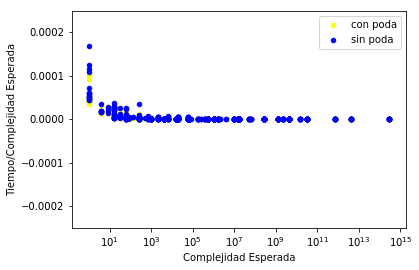
\includegraphics[width=0.4\textwidth]{complejidad1.png}
	\caption{ Gráfico de segundos de ejecución (de cada jugada) dividido $a^b$ en función de $a^b$ para los partidos jugados por el algoritmo con y sin poda en tableros pequeños contra el jugador random.}
\end{wrapfigure}


Para verificar que la poda efectivamente se ejecutaba y permitía podar varios niveles del árbol de ejecución del minimax, decidimos analizar el tiempo de ejecución ya que si no se analizaran estas partes podadas, el tiempo de ejecución sería menor. Por eso se ejecutó para exactamente las mismas partidas con las que se experimentó sin poda, la misma cantidad de veces cada una, contra el mismo jugador (que era el jugador random) que es importante aclarar que como no era determinístico medimos en la misma partida (o sea, ambos algoritmos -con y sin poda- recibían el mismo tablero a cada jugada) el tiempo de ejecución de ambos (y finalmente jugaba el ''con poda'' la jugada -lo que nos resultaba poco relevante ya que queríamos medir tiempos de ejecución para distintos tableros y verificar nuestra complejidad que no dependía de cómo jugaban y tampoco era el objetivo analizar como jugaban-). Luego se compararon los dos tiempos medidos para las 688 jugadas en todos los partidos. Así, solamente fueron 9 jugadas en las que el algoritmo con poda tardó más que el sin poda y estas diferencias fueron realmente despreciables (tanto en cantidad de jugadas diferentes, como en diferencia de tiempo). Listamos a continuación los valores en los que difirieron (5.8e-05 contra 5.6e-05, 0.000383 contra 0.000352, 0.000212 contra 0.000202, 0.000535 contra 0.000251, 0.000282 contra 0.00027, 0.00028 contra 0.000264, 0.000469 contra 0.000459, 0.000417 contra 0.000355, 0.000341 contra 0.000323 -del algoritmo con poda contra el sin poda respectivamente-).
\textbf{SI HAY TIEMPO, HACER UNA TABLITA, QUEDA MÁS FACHERO}

Esta experimentación nos permitió no solo reforzar nuestra hipótesis (justificada teoricamente en el algoritmo) de que el tiempo de ejecución era efectivamente menor, por lo que se ejecutaba la poda, sino también comprobar que se seguía manteniendo la complejidad teórica propuesta para el algoritmo con poda (ya que era la misma que la del algoritmo sin poda y hemos visto que el tiempo de ejecución era menor). Más aún esto se puede ver en la Figura 1 donde se ve que el algoritmo con poda nunca supera al algoritmo sin poda en tiempo de ejecución.



















\section{Jugador parametrizable}


\subsection{El algoritmo}
\textbf{NUEVO}
El algoritmo consiste basicamente en establecer un sistema de puntos para cada tablero, donde se miden solamente ciertas características que decidimos nosotros. A cada una de esas características se le asignara una importancia. El jugador es goloso en el proximo paso, o sea, evalúa todas las opciones que tiene para jugar (todas las columnas donde se puede jugar) y se queda con la que tenga un tablero que le da el mayor puntaje. La libertad que tiene el jugador es la importancia de cada característica, que es lo que luego se buscara optimizar. Las características que decidimos considerar fueron cantidad de fichas en la columna central, en algun borde, en alguna esquina; cantidad de fichas consecutivas de tamaño 1,2,..,c-1; cantidad de fichas consecutivas de tamaño 1,2,..,c-1 que se pueden extender;  cantidad de fichas consecutivas de tamaño 1,2,..,c-1 que se pueden extender en el próximo turno (extensiblesprox);  y cantidad de fichas consecutivas de tamaño 1,2,..,c-1 que se pueden extender en ambos sentidos (biextensibles). Cada una de estas características se considero para los dos jugadores.
\subsubsection{El Pseudocódigo}
En el \texttt{main} a la variable $movida$ se le asigna el resultado de la función \texttt{parametrizable} que es el algoritmo goloso propuesto para esta parte del problema. Esta toma los mismos parámetros que \texttt{minimax} con el agregado del \textbf{parametro} $param$ y devuelve el número de columna que se debe jugar.

La idea es que se asigne un puntaje a cada tablero y de las ocho opciones posibles se tome la de mayor puntaje (esta sería la parte golosa).

En la función se llama a la función \texttt{puntaje} que se verá luego.

La variable $tablero$ se pasa por referencia.
\begin{algorithm}

    \Function{parametrizable}{\textbf{int} rows, \textbf{int} columns, \textbf{int} c, \textbf{int} p, matriz(\textbf{int}, \textbf{int}) tablero, \textbf{int} ultimajugada, \textbf{parametro} param}
    	\State $posibles$ = [0,..,$columnas-1$] - las columnas llenas del $tablero$
    	\For{$i$ = [0,..,$\lvert posibles \rvert$)}
    		\If{jugando $posibles[i]$ se evita perder en la siguiente jugada}
    			\State \textbf{return} $posibles[i]$
    		\EndIf
    	\EndFor
    	\State \textbf{float} $maximoPuntaje$ = \texttt{puntaje}(rows, columns, c, p, tablero, posibles[0], param)
    	\State \textbf{int} $maxpos$ = $posibles[0]$
    	
    	\For{$q$ = [1,..,$\lvert posibles \rvert$)}
			\State \texttt{AgregarAtrás}($tablero[posibles[q]]$, 1)
			\If{\texttt{puntaje}($rows$, $columns$, $c$, $p$, $tablero$, $posibles[q]$, $param$)>$maximopuntaje$}
				actualizar $maximopuntaje$ y $maxpos$
			\EndIf
			\State Sacarle el último a $tablero[posibles[q]]$		
		\EndFor
		\State \textbf{return} $maxpos$
    \EndFunction

\end{algorithm}


La función \texttt{puntaje} devuelve un entero asociado a cierta jugada que se pasa por parámetro (es decir, no solo se pasa la columna donde se se juega, sino también, el tablero con las fichas). La función en sí consiste simplemente en sumar ciertos variables asociadas a características del estado actual del juego. Por ejemplo, como no es lo mismo tener una ficha en el centro que en un borde, la variable asociada a la cantidad de fichas del centro tendrá más peso que la del borde. De este modo, se cuentan ĺas distintas características del \textbf{parametro} asociadas al tablero actual tanto para el jugador 1 como para el 2. Finalmente, entonces, se devuelven las cantidades del jugador 1 y se le restan las del jugador 2 (pues son las cosas que le convienen al oponente).

Previamente se verifica si con la jugada se gana o no. Si es así, el puntaje es $\infty$ así claramente es el máximo y la función anterior lo elige como jugada.

La variable $tablero$, como en \texttt{parametrizable} también se pasa por referencia pero como \texttt{const}.
\begin{algorithm}
    \Function{puntaje}{\textbf{int} rows, \textbf{int} columns, \textbf{int} c, \textbf{int} p, matriz(\textbf{int}, \textbf{int}) tablero, \textbf{int} ultimajugada, \textbf{parametro} param}
		\If{\texttt{gane}}
			\State \textbf{return} $\infty$
		\EndIf    	
    	\State contar los que estan en el borde de cada jugador
    	\State contar la cantidad de fichas que estan en una esquina de cada jugador
    	\State contar la cantidad de fichas en el centro de cada jugador
		\State contar la cantidad de casillas libres alrededor de cada ficha de cada jugador
		\State contar la cantidad de fichas consecutivas de cada jugador
		\State contar cantidad de inmediatemente extensibles en la próxima jugada de cada jugador
		\State contar cantidad de  extensibles en cualquier momento de cada jugador
		\State contar cantidad de  bi-extensibles (extensibles en ambos sentidos) en cualquier momento de cada jugador
		\State \textbf{return} \sum cantidad$_{jugador1}*$(puntaje del parámetro)-cantidad$_{jugador2}*$(puntaje del parámetro)
    \EndFunction

\end{algorithm}

\textbf{NUEVO}
Cabe aclarar que contar la cantidad de fichas en determinadas posiciones es simplemente recorrer el tablero en busqueda de esas posiciones. De forma similar, contar las consecutivas es mirar todas las filas columnas y diagonales que hay en el tablero y recorrerlas, contando las consecutivas de un jugador (es recorrer todo el tablero 4 veces, una horizontalmente, otra vertical, una en diagonal desde arriba a la izquierda hacia abajo a la derecha y la ultima en diagonal desde arriba a la derecha hacia abajo a la izquierda). Teniendo esto en cuenta es simple chequear si cada una de estas tiras es extensible o bi extensible, viendo simplemente si sus casillas por donde podrían seguir estan vacías o no (si existen, cosa que podría no suceder en caso de estar en el borde del tablero) y para ver si son extensibles en el proximo turno es cuestion de analizar si estas casillas tienen debajo alguna ficha o son la primera de su columna (o sea si se puede jugar ahí en el próximo turno).

\subsection{Complejidad}

Veamos que el jugador que presentamos decide que jugada realizar en tiempo$\mathcal{O}(N^2 M)$ que es menor que $\mathcal{O}(N^2 M^2)$ y por ende cumple la complejidad pedida. 

En primer término, veamos que calcular el puntaje de un tablero es $\mathcal{O}(NM)$ puesto que lo único que hacemos es recorrer todas las filas, columnas y diagonales (que en total son 4 veces, no importa igualmente cuánto sino que es una cantidad constante) y en cada una de ellas contamos cuántas fichas son nuestras y cuántas de él. Pero esto lo repetimos una vez por cada parámetro que tenemos, pero como tenemos finitos (y constantes) parámetros, por lo que pasamos a recorrer una cantidad constante de veces el tablero $\mathcal{O}(c)$. Además, chequeamos si ganamos, que como ya hemos visto en la complejidad del jugador óptimo es Esto es porque recorrer el tablero es $\mathcal{O}(NM)$ ya que para cada sentido de recorrida, pasamos solo una vez por cada casilla, o sea recorremos $N*M$ casillas; repitiendo esto una cantidad constante de veces (la cantidad de parámetros) y para una cantidad constante de sentidos (cuatro) nos da que recorrimos una cantidad constante de veces $N*M $ casillas, por lo que la complejidad de calcular el puntaje es efectivamente $\mathcal{O}(NM)+\mathcal{O}(c)=\mathcal{O}(NM)$ puesto que $c<\min{N,M}$.

Cabe aclarar aquí que consideramos como un parámetro a los vectores de parámetros (como es el caso de consecutivos) ya que para ellos recorremos solo cuatro veces el tablero (en todos los sentidos) y lo que cambia es dónde alojamos cada valor del vector según cuántas consecutivas encontremos del mismo color. Cabe aclarar también que la operación para saber qué ficha está en una casilla es $\mathcal{O}(1)$ porque guardamos al tablero en una matriz, esto es fundamental para poder asegurar la complejidad pedida.

 
Pero nuestro jugador no hace solo eso, sino que analiza cómo quedaría el puntaje del tablero para cada una de sus $N$ posibles jugadas y luego se queda el máximo de ellas (esta es la parte golosa). Repite entonces $N$ veces algo  $\mathcal{O}(N M)$ por lo que da una complejidad de $\mathcal{O}(N^2 M)$ y luego calcula el máximo sobre $N$ elementos que suma $\mathcal{O}(N)$ (es recorrer linealmente un vector) y da una complejidad total de $\mathcal{O}(N^2 M) +\mathcal{O}(N) = \mathcal{O}(N^2 M)$.

\subsection{Experimentación}


\begin{wrapfigure}{L}{0.4\textwidth}
	%\centering
	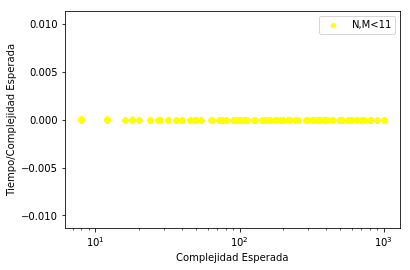
\includegraphics[width=0.4\textwidth]{complejidad2.png}
	\caption{ Gráfico de segundos de ejecución (de cada jugada) dividido $N^2 *M$ en función de $N^2 * M$ para los partidos jugados por el jugador que utiliza la función parametrizable a cada paso. Varian $c$ y $p$. Columnas y filas menores a 11.}
\end{wrapfigure}

Si bien el grueso del análisis y experimentación sobre este jugador consistirá en buscar buenos parámetros que mejoren al jugador, consideramos relevante reforzar experimentalmente nuestra hipótesis de complejidad teórica esperada. Para esto tomamos mediciones análogas a las del jugador óptimo solo que jugando en más tableros. Se jugó en tableros que comprendían todas las combinaciones factibles con las columnas y filas moviéndose entre $2$ y $10$, $c$ moviendose entre $2$ y $\min{columnas,filas}$ y $p$ moviéndose entre $2$ y $filas*columnas/2$. En cada jugada, los parámetros que determinaban la próxima jugada a realizar se sorteaban aleatoriamente. Todo esto fue para ver experimentalmente que la dependencia que proponíamos en la complejidad dependía efectivamente solo de $n$ y $m$. Así, igual que antes, realizamos un gráfico de tiempo de ejecución/(filas*columnas$^2$) en función de filas*columnas$^2$ donde esperábamos obtener un gráfico constante que reforzaría nuestra hipótesis de que la complejidad (como se justificó teóricamente) era de $\mathcal{O}(N^2 M)$. Este gráfico se puede ver en la Figura 2.




Efectivamente, como se puede ver en la Figura 2, pareciera cumplirse la complejidad esperada ya que el gráfico es practicamente constante. Más aún, al variar por todas sus posibilidades $c$, $p$ y el parámetro de la función, esto refuerza la hipótesis (que se justificó en la explicación del algoritmo) de que esta cota de dependencia no se ve afectada por el parámetro en particular, o la cantidad de fichas que queden, o el $c$. Sabiendo esto, tenemos la posibilidad de experimentar para tableros de mayor tamaño (ya que no tenemos que repetirlos para distintos $c$ y $p$). Por esto, se experimentó con un $c$ aleatorio (con distribución uniforme, usando \texttt{rand()} de C++) entre 2 y $\min{columns,rows}$, y $p=N*\frac{M}{2}$ para que no se interrumpa el partido por falta de fichas y se varió nuevamente las filas y columnas pero ahora el límite superior paso a ser 20 en vez de 10. Nuevamente, se realizó el mismo gráfico que antes con los nuevos datos que se puede ver en la Figura 3.

\begin{wrapfigure}{R}{0.4\textwidth}
	%\centering
	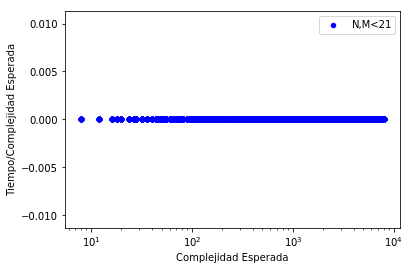
\includegraphics[width=0.4\textwidth]{complejidad2b.png}
	\caption{ Gráfico de segundos de ejecución (de cada jugada) dividido $N^2 *M$ en función de $N^2 * M$ para los partidos jugados por el jugador que utiliza la funcion parametrizable a cada paso. Columnas y filas menores a 51.}
\end{wrapfigure}

Podemos ver en el gráfico de la Figura 3, que los resultados siguen siendo los mismos incluso para tableros de tamaño mayor. Nuevamente el gráfico es prácticamente una constante. El análisis y su justificación es totalmente análogo al realizado en la Figura anterior (la 2) y al ser con tamaños de entrada mayores, refuerza más aún experimentalmente la complejidad que fue propuesta teóricamente.






\section{Grid Search}



\subsection{El algoritmo}

\subsubsection{El Pseudocódigo}





\subsection{Experimentacion}

\subsubsection{Primera exploración}

A causa de la cantidad de parámteros (ya son 28 para el 4 en línea) que tiene en cuenta la función paramétrica detallada en la sección 3, resulta demasiado costoso computacionalmente explorar todo el espacio de posibilidades con un grid search clásico. Incluso  con una granularidad muy baja, comparando entre tan poco como 20 valores posibles para cada parámetro (cada uno en [-1,1] con saltos de 0,1) se deben analizar $ 20^{28}$ combinaciones de parámetros distintas.

A causa del tamaño inabarcable del espacio de búsqueda se decidió entonces utilizar un método que reduce de forma drástica el tiempo necesario para obtener resultados del grid search, con el conocimiento de que no se podrá explorar todo el espacio de esta forma. Empezando con un conjunto de parámetros aleatorios se buscaba con el método de grid search la configuración óptima únicamente para los primeros dos parámetros. Una vez que se encontraron los valores óptimos para los primeros dos parámetros en el contexto del conjunto aleatorio inicial, se procede a optimizar el próximo par de parámetros pero manteniendo los mejores valores encontrados para el par ya explorado. Esto se repite hasta que se optimizaron todos los parámetros a tener en cuenta. La desventaja de este método es que a medida que se van modificando los valores de pares, las optimizaciones iniciales van perdiendo relevancia, ya que pueden no ser las óptimas para esta nueva configuración.

Este primer intento no dio buenos resultados, el jugador resultante no realizaba las jugadas esperadas y no podía reconocer ni siquiera instancias en las que estaba a un turno de perder y podía salvarse.


\subsubsection{Modificaciones}

En busca de mejores resultados se realizaron los siguientes cambios para mejorar el conjunto de parámetros resultante de ejecutar el \textit{grid search} con un jugador inicial aleatorio al cual se le van optimizando un par de parámetros a la vez. El primer cambio fue simplemente iterar la versión anterior varias veces, aprovechando que recorrer matrices de sólo 2 dimensiones hace al algoritmo más rápido. Como siempre se guarda el mejor jugador hasta el momento y se lo suplanta únicamente si se encontró otro conjunto de parámetros mejor, realizar más iteraciones en el peor caso mantendría la misma solución. El objetivo de este cambio sería darle otra oprtunidad a los parámetros a optimizarse en este nuevo contexto en el cual las otras preferencias del jugador no son las iniciales aleatorias, sino unas calculadas en base a este mismo algoritmo. 

Otra modificación fue poner los parámetros que consideramos más importantes (la cantidad de filas biextensibles grandes por ejemplo) más adelante en el orden en que se chequean, es decir que se optimicen primero, antes de tocas los otros parámetros aleatorios. De esta forma se busca dejarlos buscar su configuración óptima sin estar condicionados por los valores convenientes para otros parámetros menos importantes.



\subsubsection{Grid recomendado}

Incluso con las modificaciones a la idea original, la forma de recorrer la grilla de a pares de parametros resultaba muy acotada, y no llegaba a encontrar buenas combinaciones de valores que resultaran en un jugador bueno. Esto es de esperar ya que si recordamos el tamaño gigante de $ 20^{28}$ posibilidades no hay manera de explorarlo bien en un tiempo razonable. A causa de esto se recurrió a la posibilidad de comenzar el grid search no con un conjunto de parámetros aleatorios, si no con un jugador hecho "a mano", con parámetros medianamente buenos. Con esto se buscaba que el grid search explore opciones cercanas a un conjunto que ya se sabe no es muy malo, de esta forma se intentó evitar la gran cantidad de combinaciones inútiles que el algoritmo estaba recorriendo previamente, y en su lugar mejorar una solución inicial.

Con esta recomendación de parámetros iniciales ya sí se pudieron observar resultados interesantes del grid search. El jugador resultante surge de haber vencido a los valores de entrada, por lo cual no sólo tiene un nivel de juego muy superior a los intentos previos del algoritmo, además mejora por sobre los parámetros de entrada, de forma que finalmente se logró llegar a un algoritmo de optimización de búsqueda por metodo de grid search que efectivamente logre encontrar una solución buscada.

Como conclusión se pudo concluir que a causa del inmenso espacio de búsqueda resultaba inviable la exploración no asistida del mismo, por esto se recurrió (y se constató que es una alternativa efectiva) a comenzar la exploración desde un punto de partida bueno e ir mejorando el conjunto de parámetros a partir de este input con valores (PALABRA DE QUE LOS SELECCIONAMOS A MANO, PERO PODRIAN HABER SIDO OTROS. COMO ERAAAAA)











\section{Algoritmo Genético}

El algoritmo genético se basa en la teoría genética darwiniana y busca básicamente recrear la evolución de una población. Los individuos más aptos tendrán mayor probabilidad de perdurar a lo largo de las generaciones, transmitiendo así los genes que hacen que sean más aptos. Se recrea también la mutación que permite que haya cambios en los genes (que pueden ser beneficiosos para la aptitud como no) de forma aleatoria. También se da el \textit{crossover}, donde los genes de uno de los individuos se cruza con los de otro, generando así nuevos individuos que no son copia de uno ni de otro sino una mezcla de ambos. Para mayor precisión, a continuación se encuentra el pseudocódigo. Solo hay que hacer una salvedad previa: para medir qué individuo es mejor que otro, se usaron dos funciojnes distintas de \textit{fitness}, una de las cuales usa como parámetro un entero $k$.

\subsubsection{El Pseudocódigo}
\begin{algorithm}
\caption{genetico}
\begin{algortithmic}[1]
	\Function{genetico}{\textbf{int} rows, \textbf{int} columns, \textbf{int} c, \textbf{int} p}
	\State \textbf{int} $tamanopoblacion$, $totalgeneraciones$, $k$
	\State \textbf{float} $min$, $max$, $pmutar$, $pcrossover$
	\State vector(\textbf{parametro}) $poblacion$ = vector de longitud $tamanopoblacion$ donde cada elemento está dado por sendos llamados a \texttt{paramrandom}($c$)
	\For{$generacion$ = [1..$totalgeneraciones$)}
		\State poblacion = \texttt{seleccion}
		\For{$i \in poblacion$}
			\State \texttt{mutar}($i$) con probabilidad $pmutar$
		\EndFor
	\EndFor
	\State \textbf{float} $maximo$ = \texttt{fitness}($poblacion[0]$, $poblacion$, $rows$, $columns$, $c$, $p$)
	\State \textbf{int} $maxpos$ = 0
	\For{\textbf{int} $i$ = [1..$poblacion$)}
		\State \textbf{float} $actual$ = \texttt{fitness}($poblacion[i]$, $poblacion$, $rows$, $columns$, $c$, $p$)
		\If{$actual>maximo$}
			\State actualizar $maxpos$ y $maximo$
		\EndIf
	\EndFor
	\State \textbf{return} $poblacion[maxpos]$
    \EndFunction
\end{algortithmic}
\end{algorithm}

En el pseudocódigo anterior se hicieroN llamadas a las siguientes funciones:

\begin{itemize}
\item \texttt{paramrandom}: asigna aleatoriamente un número entre -1 y 1 a cada parámetro
\item \texttt{seleccion}: \textbf{ESTOY PONIENDO LA 2} para todos los individuos, toma otros al azar, elige al mejor y lo cruza con otro elegido de la misma forma. Repite este proceso hasta tener todos los que queremos. Además, sigue el principio del elitismo, es decir, conserva siempre al mejor individuo copiándolo tal cual.
\item \texttt{mutar}: para cada parámetro, si un número aleatorio entre 0 y 1 es menor que la probabilidad de mutar $pmutar$ entonces se vuelve a randomizar ese parámetro.
\item \texttt{fitness}: 
\end{itemize}

\textbf{NUEVO}

Como muestra el pseudocódigo, el algoritmo lo que hace es establecer un tamaño de población e inicializa de alguna manera (en principio de forma aleatoria) a todos estos individuos. En nuestro caso, nuestros individuos son una estructura que contiene un valor particular para cada uno de los parámetros que tomaba la funcion del jugador parametrizable.

Hasta que se cumpla una condicion de corte (en principio una cantidad fija de generaciones, pero esta variará también siendo un tiempo, o podría ser también cierta condicion de convergencia), se generarán nuevas poblaciones, que serán la próxima generacion. Cada generación sufre un proceso de mutación y para dar lugar a una nueva, se da un proceso de selección que determina pares de individuos con los cuales se realizará el crossover dando lugar asi a un nuevo individuo que será parte de la próxima generación.

Para decidir a que individuos seleccionar, se utiliza una función de fitness que basicamente decide (de alguna forma) cuan apto es un individuo. A partir de estos valores, el proceso de selección decidirá quienes seran los que darán lugar a la nueva generacion (en general, los más aptos son los que tienen mas probabilidad de dar descendencia, ya que sus genes dan individuos más aptos).

A lo largo de toda la experimentación utilizamos diversas funciones de estas que detallamos a continuacion

\begin{itemize}
\item \textbf{\underline{Crossover:}} Consiste en dados dos individuos (padres, dos estructuras de parámetros), generar un nuevo individuo que cada gen (cada parámetro particular) sea o bien de un padre o bien del otro. En nuestro caso toma un valor pcrossover que indica la probabilidad de que se cambie el padre del cual se estan copiando los genes. El primer gen lo copia del primer padre pasado por parámetro, y cada vez que va al siguiente gen, sortea un numero (con una función random de distribución uniforme, rand() de C++) en $[0,1]$ y si el resultado cae en $[0,pcrossover]$ copia el siguiente gen del otro padre y sino sigue copiando del mismo. En principio, como los vectores que son parámetros (extensibles, extensiblesprox, biextensibles, consecutivos) presentan una clara relación entre ellos decidimos que sean tomados como un gen entero (o bien se copia el vector de un padre o bien del otro)

\item \textbf{\underline{Mutación:}} Consiste en dado un individuo, cambiar cada uno de sus genes en base a alguna distribución de probabilidad. En nuestro caso, la funcion tomaba un valor pmutar. De forma análoga al crossover para cada gen se sorteaba un numero y si caía en $[0,pmutar]$ ese gen mutaba y pasaba a tomar un nuevo valor aleatorio (generado con la funcion rand() de C++) entre un valor min y max que eran los valores minimos y máximos que podía tomar el puntaje.


\item \textbf{\underline{Selección 1:}} Consiste en calcular el fitness de todos los individuos de la población y para los que esten en una proporcion de los que tienen mas fitness (se fijo inicialmente en la mitad con más fitness) tomar dos aleatoriamente (con distribución uniforme, usando rand() de C++) y a esos aplicarles crossover obteniendo así un individuo de la nueva poblacion. Repetimos este proceso de tomar dos aleatoriamente de ese grupo hasta que la nueva población tenga el mismo tamaño que la anterior. Siempre se incluye tal cual estaba en la nueva generación al mejor de la anterior (esto es elitismo, propiciamos que el mejor de todos se mantenga). Notar que si bien siempre se deja como estaba, este individuo (si no lo evitamos) podría sufrir alguna pequeña mutación.

\item \textbf{\underline{Selección 2:}} Consiste en generar grupos de un cierto tamaño (que se fijo inicialmente en el 20\% de la poblacion) tomando a sus integrantes de toda la población (con distribución uniforme, usando rand() de C++). Luego dado un grupo se elegía al mas apto dentro de ese grupo (al que tuviera mayor fitness), se repetía lo mismo obteniendo un segundo individuo (obtenido desde un nuevo grupo) y luego se realizaba crossover con estos dos obteniendo un individuo de la nueva generacion. El proceso se repetía hasta que la nueva generación tuviera el mismo tamaño que la anterior. Nuevamente se utilizó elitismo, dejando en la nueva población tal cual estaba al mejor de la anterior

\item \textbf{\underline{Fitness 1:}} Se hace jugar a cada individuo contra todos los de su poblacion dos partidos, donde en uno empieza y en el otro va segundo. Se cuenta la cantidad de partidos en los que no perdió y se los divide por la cantidad de partidos jugados para normalizarlos (queda el fitness en [0,1] y además permite que quede en el mismo rango para disintos tamaños de población).


\item \textbf{\underline{Fitness 2:}} La idea de esta función de fitness es establecer un sistema de puntos. Nuevamente se hace jugar a cada individuo contra todos los de su población dos partidos, donde en uno empieza y en otro va segundo. Se da un puntaje según pierda gana o empata (pierde=0; empata=5; gana=10) y se da un bonus si se empieza segundo ya que suponemos que en tableros medianamente grandes es una ventaja comenzar (BonusPierde=1; BonusEmpata=2; BonusGana=4). Luego, se divide al puntaje sobre la cantidad de partidos jugados (para poder tener los mismos valores de fitness en poblaciones de distintos tamaños).
\end{itemize}


\subsection{El algoritmo}



\subsection{Experimentacion}

Para comenzar con la experimentación, tratamos de comprender como influían los métodos de seleccion, funciones de fitness, crossover y mutación para así luego buscar la mejor forma de utilizar el algrotimo genético en nuestro caso. Para esto comenzamos estudiando estas funciones del algoritmo genético en el 4 en línea por ser una instancia particular que no es pequeña (tiene un tamaño considerable para ver diversas estrategias), ni es muy grande (los tiempos para experimentar son abarcables) pero podríamos haberlo hecho con cualquier otra sin problema.


Primeramente, tratamos de comprender como afectaría el tamaño de las poblaciones. Si bien una población grande tiene como ventaja aportar mucha mas variedad genética, los tiempos de ejecución son mucho mayores. Por su parte, una población pequeña si bien tiene poca variedad genetica, da muchísismas más generaciones en la misma cantidad de tiempo. Se buscó entender que tipo de poblaciones brindaban mejores jugadores en el mismo tiempo. También se busco encontrar que fitness brindaba mejores jugadores y como eran las características de los métodos de seleccion.

Es por esto que se corrio el algoritmo genético para ambos métodos de seleccion y ambas funciones de fitness durante dos horas y media con poblaciones grandes, intermedias y chicas (de 100, 50 y 10 individuos cada una). Las poblaciones se inicializaron de forma aleatoria, donde cada parámetro se inicializaba de forma aleatoria como un float entre -1 y 1 (con distribucion uniforme, se utilizo la funcion rand() de C++). Las poblaciones de 100 individuos dieron 10 generaciones, las de 50 individuos dieron 37 y las de 10 individuos dieron 750 generaciones en el tiempo indicado. En todos estos casos, la probabilidad de mutar se fijo en 0.005 y la de crossover en 0.4




\begin{figure}[H]
	\captionsetup[subfigure]{position=b}
	\centering
	\subcaptionbox{tamaño 10}{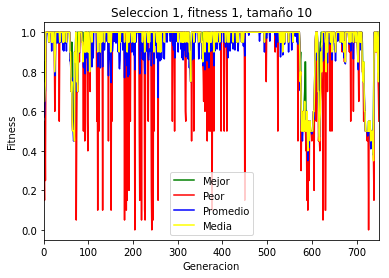
\includegraphics[width=0.3\linewidth]{s1f1t10.png}}
	\subcaptionbox{tamaño 50}	{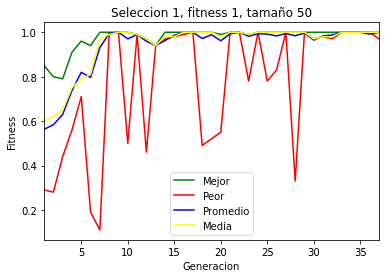
\includegraphics[width=0.3\linewidth]{s1f1t50.png}}
	\subcaptionbox{tamaño 100}{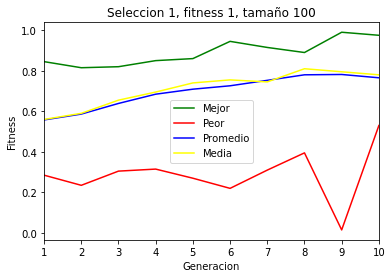
\includegraphics[width=0.3\linewidth]{s1f1t100.png}}
	\caption{Gráfico de fitness en funcion de generación. Se gráfica el mejor, peor, la media y el promedio. Seleccion 1, fitness 1, pmutar=0.005 pcrossover=0.4}
\end{figure}

Como podemos observar en la figura 4, efectivamente a mayor tamaño de población menor es la cantidad total de generaciones que se generan en el mismo tiempo (2.5 horas). Tanto en la figura 4.a) y 4.b) podemos ver que hay momentos en los que la población pareciera converger, o sea, tanto el mejor, peor, promedio y media valen 1, que es el máximo valor de fitness que pueden tomar (recordamos que estamos utilizando fitness uno que es la proporcion de partidos no perdidos sobre el total). En ambas, esta situación no se mantiene por el resto de las generaciones ya que hay mutaciones que perturban esta situación. Sin embargo es notable que en todos los casos la media sigue manteniendose muy alta (casi 1, que es el valor maximo) a pesar de haber mutaciones (a excepcion de la mutación que se ve en la figura 4.a) al rededor de la generación  100, 600 y 700). Además de la media, el mejor sigue también manteniendose en valores máximos (a excepcion de las mutaciones mencionadas). Esto puede suceder gracias al elitismo, puesto que aseguramos que el mejor individuo de la generacion pasada se incluya en la nueva generacion asi como esta, sin ser modificado. Estas situaciones en las que cambia el mejor y la media, podrían ser en las que el mejor individuo muta. La otra opcion sería que aparece un nuevo individuo que es no es ni mejor que el que era el mejor ni peor, o sea, a veces le gana y a veces pierde, por lo que ambos no tienen fitness máximo. Esto último pareciera ser menos factible ya que no debería descender tanto la media por solamente un individuo así, a menos que sean varios, lo que es verdaderamente muy poco probable (ya es poco probable que varios muten considerablemente).

La convergencia de la media a un valor cercano al máximo de fitness pareciera ser rápida, en el caso de poblacion de tamaño 50 se da alrededor de la generación 10. En el caso de la de tamaño 10 se da tan solo en la quinta generacion. Esto tiene sentido ya que es menor el tamaño de la población. Por último, en las 2.5 horas transcurridas, se ve un claro aumento de la media en la población de tamaño 100, pero no llegó aún a converger en dicho tiempo.

Más aún cabe notar que una mutación en una población pequeña la afecta mucho (porque es una cantidad de genes mucho mas significativa respecto del total) más que en una población grande.Estos gráficos ayudan claramente a reforzar dicha hipótesis. Esto se puede ver ya que las variaciones repentinas, a mayor tamaño de poblacion son más suaves, ya que en el grafico de la figura 4.a) podemos ver picos muy acentuados en los que desciende hasta por debajo de 0.8, situación que en la figura 4.b) no desciende por debajo de 0.9 siquiera-una vez que convergió- y si observamos la figura 4.c) vemos que la media siempre aumenta, a excepcion de en la generacion 7 donde disminuye casi despreciablemente. 

Cabe destacar que esta poca variabilidad que hay en la funcion de fitness y la rápida convergencia se puede deber no solo a que se tratan por igual las victorias y empates, tanto se empiece o no, sino también a que el método de selección solamente toma los genes de los mejores individuos (de la mitad superior), por lo que la variabilidad es menor. Para tratar de comprender mejor esto, se realizó la misma experiencia con la funcion de fitness2, que distinguía empates de victorias y quien comenzaba.





\begin{figure}[H]
	\captionsetup[subfigure]{position=b}
	\centering
	\subcaptionbox{tamaño 10}{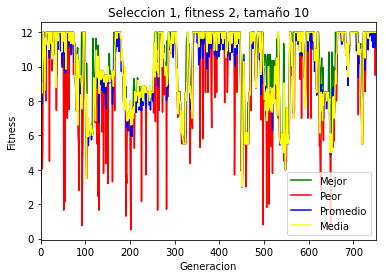
\includegraphics[width=0.3\linewidth]{s1f2t10.png}}
	\subcaptionbox{tamaño 50}	{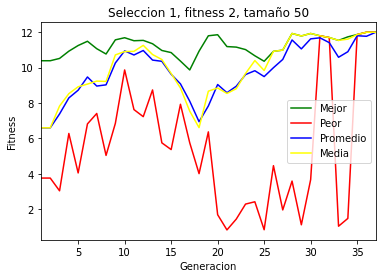
\includegraphics[width=0.3\linewidth]{s1f2t50.png}}
	\subcaptionbox{tamaño 100}{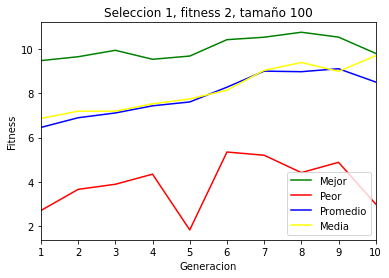
\includegraphics[width=0.3\linewidth]{s1f2t100.png}}
	\caption{Gráfico de fitness en funcion de generación. Se gráfica el mejor, peor, la media y el promedio. Seleccion 1, fitness 2, pmutar=0.005 pcrossover=0.4}
\end{figure}

Efectivamente como podemos ver en la figura 5, la variabilidad aumenta mucho más al cambiar la función de fitness como esperabamos ya que esta distingue muchas más situaciones (distingue empates de victorias y distingue si uno empieza o no). Para todos los tamaños de población la media sufre alteraciones mayores en comparacion con la media de su gráfico análogo con la otra funcion de fitness.

Algo destacable de esta funcion de fitness es que las mutaciones y cambios en generaciones modifican el fitness del mejor, que disminuye varias veces bastante (cosa que practicamente no sucedia con la anterior funcion de fitness -ver Figura 4-). Esto ultimo sucede porque el fitness depende mucho más del resto de los jugadores porque considera más situaciones. Además la convergencia sucede varias generaciones despues que con la primer funcion de fitness (en el caso de poblacion 50 se puede ver una convergencia recien en las ultimas generaciones, las mayores a 30, mientras que con la otra funcion de fitness era a la decima generacion). 

Analizando el gráfico 5.a) podemos ver que las mutaciones afectan mucho más al fitness ya que la media desciende considerablemente, llegando a la mitad de su valor máximo en reiteradas ocasiones.Nuevamente podemos observar que las mutaciones afectan mucho más en poblaciones pequeñas, como se observaba en la figura 4.

Teniendo entonces un análisis de la interacción entre la selección 1 con los dos fitness, repetimos el análisis pero con la seleccion 2.



\begin{figure}[H]
	\captionsetup[subfigure]{position=b}
	\centering
	\subcaptionbox{tamaño 10}{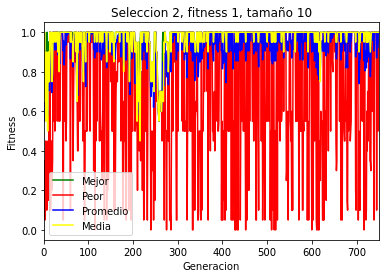
\includegraphics[width=0.3\linewidth]{s2f1t10.png}}
	\subcaptionbox{tamaño 50}	{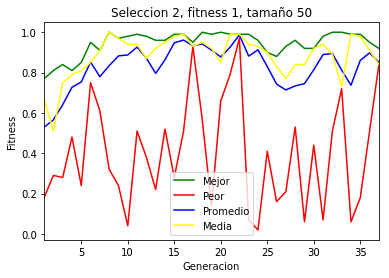
\includegraphics[width=0.3\linewidth]{s2f1t50.png}}
	\subcaptionbox{tamaño 100}{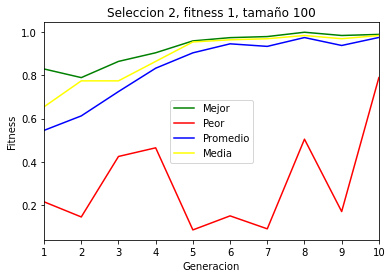
\includegraphics[width=0.3\linewidth]{s2f1t100.png}}
	\caption{Gráfico de fitness en funcion de generación. Se gráfica el mejor, peor, la media y el promedio. Seleccion 2, fitness 1, pmutar=0.005 pcrossover=0.4}
\end{figure}


\begin{figure}[H]
	\captionsetup[subfigure]{position=b}
	\centering
	\subcaptionbox{tamaño 10}{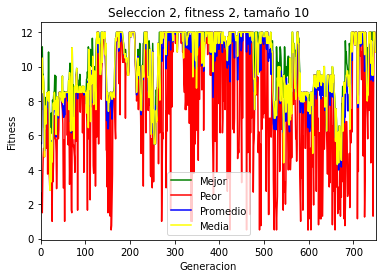
\includegraphics[width=0.3\linewidth]{s2f2t10.png}}
	\subcaptionbox{tamaño 50}	{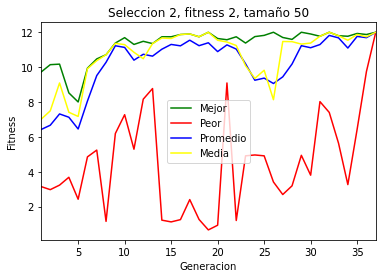
\includegraphics[width=0.3\linewidth]{s2f2t50.png}}
	\subcaptionbox{tamaño 100}{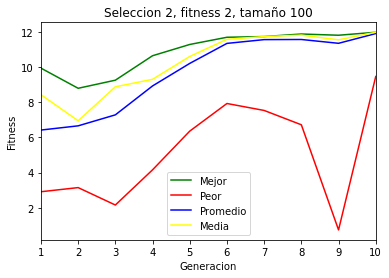
\includegraphics[width=0.3\linewidth]{s2f2t100.png}}
	\caption{Gráfico de fitness en funcion de generación. Se gráfica el mejor, peor, la media y el promedio. Seleccion 2, fitness 2, pmutar=0.005 pcrossover=0.4}
\end{figure}

En la Figura 6 y 7 podemos ver características que refuerzan que ciertas situaciones se daban segun lo conjeturado. Por ejemplo, nuevamente vemos que el fitness 2 da mayor variabilidad y reduce mas veces el fitness del mejor. Nuevamente podemos ver también que la convergencia es más rápida con la funcion de fitness 1, reforzando la hipótesis de que es porque esta considera menos situaciones (no distingue victoria de empate ni si empiezo o no).

Por último, una importante diferencia entre los gráficos con distintos métodos de seleccion es que los que usan el segundo método peor caso con mucho menor fitness y más variabilidad. Esto tiene sentido, ya que en el método de seleccion 1 solo se reproducían los que eran del 50 \% con mejor fitness, mientras que en el método de seleccion 2 se puede reproducir cualquiera de los que esten en el 80  \% de mejor fitness (ya que el torneo era de tamaño del 20  \% de la poblacion y el 20  \% peor nunca podría ganar alguno). En este sentido, la seleccion 2 si bien aporta más variabilidad, tiene peores jugadores.


Tras este análisis, tratamos de entender como afectaban las dos variables que quedaban por ver, que eran el porcentaje de mutación y el de crossover. Para ver como afectaba la probabilidad de mutación, ejecutamos con el primer metodo de selección ya que es el que proveía menor variabilidad genética y perimtiría visualizar mejor como afecta el porcentaje de mutación. También se utilizo la primer funcion de fitness por el mismo motivo. Por esto se ejecuto durante 5 horas, la población de tamaño 50 (intermedia, para tener una cantidad considerable tanto de generaciones como de individuos en la poblacion) con diferentes probabilidade de mutar, con pmutar=0.00001, 0.005, 0.01, 0.05 y 0.1. El crossover se fijo en 0.4


\begin{figure}[H]
	\captionsetup[subfigure]{position=b}
	\centering
	\subcaptionbox{pmutar 0.00001}{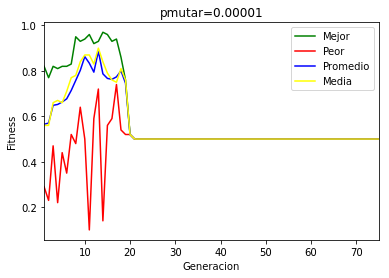
\includegraphics[width=0.3\linewidth]{muta0.png}}
	\subcaptionbox{pmutar 0.005}	{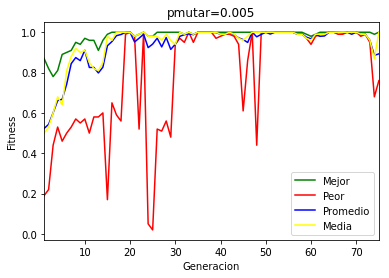
\includegraphics[width=0.3\linewidth]{muta1.png}}
	\subcaptionbox{pmutar 0.01}{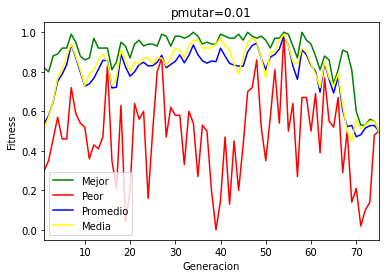
\includegraphics[width=0.3\linewidth]{muta2.png}}
	\subcaptionbox{pmutar 0.1}{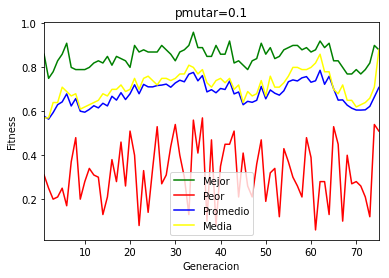
\includegraphics[width=0.3\linewidth]{muta3.png}}
	\caption{Gráfico de fitness en funcion de generación. Se gráfica el mejor, peor, la media y el promedio. Seleccion 1, fitness 1, pcrossover=0.4}
\end{figure}

La figura 8 refleja claramente lo esperado. En nuestro algoritmo genético hay operaciones que favorecen la convergencia, como es el proceso de seleccion y crossover y hay en oposición operaciones que favorecen la divergencia como es el caso de la mutación, lo que se puede ver claramente en esta figura. Con menores probabilidades de mutación, la convergencia no solo es mas rapida, sino que los cambios en el fitness una vez que convergio la población (momentos donde cambia la media) son cada vez menos. En la figura 8.d) podemos ver que hay bastantes picos, tanto en la media como en peores mejores y promedio, esto es porque la probabilidad de mutación es altísima (es un 10 \% para cada gen y hay 28 genes por individuo en este tablero) por ende es muy probable que todo individuo mute. En la figura 8.c) la situación es la misma ya que un 1 \% para cada uno de los 28 genes sigue siendo bastante alto (cada individuo tiene un 25 \% de mutar que es es $1- (0.99)^28$ o sea la probabilidad del complemento que es que no haya mutacion en ninguno de los 28 genes). En estas dos figuras no se llega a ver una convergencia en las generaciones que se dieron (podemos conjeturar que un porcentaje de mutacion tan alto no va a permitir esta convergencia). Ya en la figura 8.b) podemos ver que hay  efectivamente convergencia pero como sigue habiendo un porcentaje considerable de mutación, hay generaciones donde se sale de este pico un poco (en algunas desciende un poco la media, en otras solo desciende el peor). Finalmente en la figura 8.a) vemos una convergencia mucho mas rápida y una vez que esta se dio, todos los fitness se mantienen asi durante más de 50 generaciones, esto es porque al poner una probabilidad tan baja, la mutación practicamente no sucede y no hay otras operaciones que permitan divergencia.

Por otro lado, la selección y el crossover son operaciones que favorecen y buscan la convergencia. Para ver la influencia de la variable restante, el pcrossover, se ejecuto durante 5 horas,  para la población de tamaño 50 (intermedia, para tener una cantidad considerable tanto de generaciones como de individuos en la poblacion) con diferentes probabilidades de mutar, con pcrossover= 0.4, 0.1, 0.01, 0.00001.  El pmutar se fijo en 0.005


\begin{figure}[H]
	\captionsetup[subfigure]{position=b}
	\centering
	\subcaptionbox{pcrossover 0.00001}{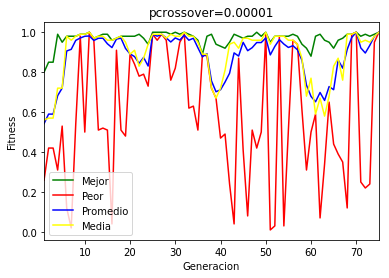
\includegraphics[width=0.3\linewidth]{crossover00.png}}
	\subcaptionbox{pcrossover 0.01}{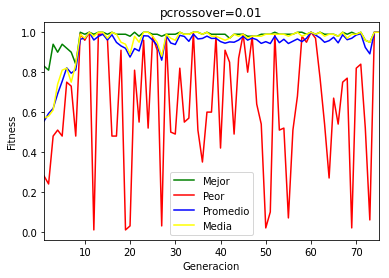
\includegraphics[width=0.3\linewidth]{crossover0.png}}
	\subcaptionbox{pcrossover 0.1}	{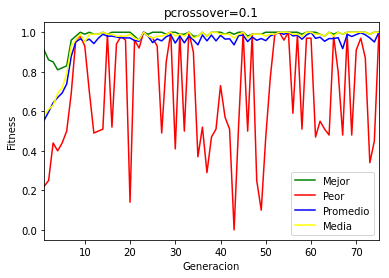
\includegraphics[width=0.3\linewidth]{crossover1.png}}
	\subcaptionbox{pcrossover 0.4}{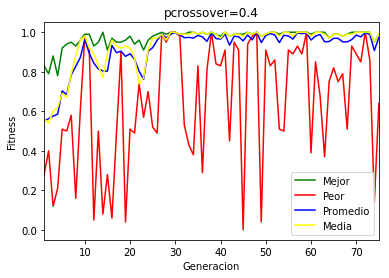
\includegraphics[width=0.3\linewidth]{crossover2.png}}
	\caption{Gráfico de fitness en funcion de generación. Se gráfica el mejor, peor, la media y el promedio. Seleccion 1, fitness 1, pmutar=0.005}
\end{figure}

Como podemos ver en la Figura 9, en contra de lo esperado, pareciera no haber una convergencia más rápida si aumentamos pcrossover. Sin embargo, considerando que la probabilidad es para cada uno de los genes, la probabilidad de crossover de 0.4 resulta altisima (considerando que para esta instancia de tablero particular hay 28 parametros), por lo que los individuos mezclan demasiado sus genes, tardando mucho más en converger que en el resto. Por otra parte, reforzando la hipotesis de que favorece la convergencia, si vemos algo con pcrossover realmente bajo como es el caso de 0.00001 en comparacion con 0.01 la convergencia es más lenta una vez que se sale de esta (la media desciende mucho más y tarda más en tomar nuevamente el valor de convergencia).

Quizás algo que pueda estar influyendo es que primeramente decidimos dejar a los vectores como una unidad, como todo un gen que se transmitía o bien de un padre o del otro. Por ende, realizamos la misma experiencia solo que ahora se decidía de que padre copiar cada uno de los elementos del vector segun pcrossover, o sea con este cambio el hijo puede tener una parte de un vector de uno y la otra parte del otro.

\begin{figure}[H]
	\captionsetup[subfigure]{position=b}
	\centering
	\subcaptionbox{pcrossover 0.00001}{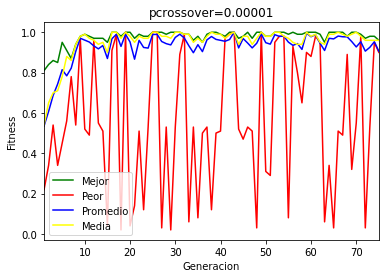
\includegraphics[width=0.3\linewidth]{crossoverB00.png}}
	\subcaptionbox{pcrossover 0.01}{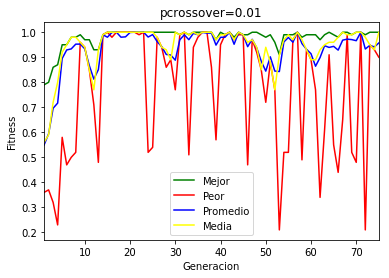
\includegraphics[width=0.3\linewidth]{crossoverB0.png}}
	\subcaptionbox{pcrossover 0.1}	{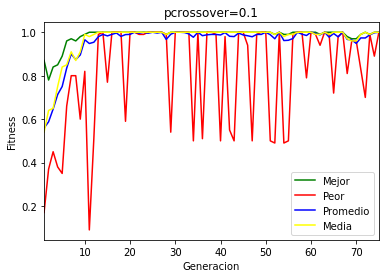
\includegraphics[width=0.3\linewidth]{crossoverB1.png}}
	\subcaptionbox{pcrossover 0.4}{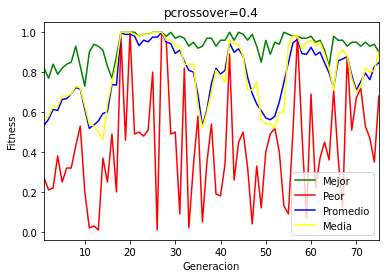
\includegraphics[width=0.3\linewidth]{crossoverB2.png}}
	\caption{Gráfico de fitness en funcion de generación. Se gráfica el mejor, peor, la media y el promedio. Seleccion 1, fitness 1, pmutar=0.005}
\end{figure}

Este cambio no pareciera sin embargo reflejar algo muy distinto, la unica diferencia es que aporta un poco más de variabilidad en todos los casos salvo en el grafico 10.c). Tiene sentido que aporte más variabilidad debido a que los individuos mezclan sus genes mucho más, dando lugares a nuevas posibilidades de valores de los vectores que son parámetro, cosa que antes solo se daba con mutaciones eventuales.

Sin embargo, con este cambio también, podemos notar que no hay influencia en la velocidad de convergencia por parte de la probabilidad de crossover, contrariamente a como esperabamos que sea al principio. Esto podría ser debido a que los parámetros, al ser la importancia de cada cosa, son bastante independientes entre sí y no tenemos bloques grandes que esten correlacionados entre sí en cuanto al juego (a lo sumo los pares que determinan mi importancia respecto de la del otro), por lo que no es tan relevante si copiamos toda una tira de parámetros de un mismo padre. Esta idea surge al ver que no pareciera haber cambios en la velocidad de convergencia cuando rompimos esas tiras (lo que graficamos en la Figura 10).

Sí en cambio resulta importante para dar más variabilidad y evitar que se la media se quede en valores cercanos al de convergencia como claramente se puede ver que sucedió en el gráfico d) de la Figura 10 donde además de ser alta la pcrossover, usamos la segunda forma donde miramos como gen heredable de algun padre a cada elemento del vector y no a este en su totalidad.

Habiendo estudiado entonces la influencia de los distintos parámetros, tratamos de buscar una combinación de estos que de un buen jugador. Todos los jugadores que fueron generados al final (el mejor de la ultima generacion para cada experimento) compitieron entre ellos.

En los primeros experimentos con 2.5 horas, para cada función de fitness y cada método de selección, hicimos competir a los tres jugadores todos contra todos dos partidos, donde se alternaba quien comenzaba. Para el método de selección 1, con ambas funciones de fitness resultaron ganadores siempre los segundos jugadores y después se vió que jugaban practicamente partidos similares donde jugaban en las casillas de mas cercanas al borde. Como reflejaban los parámetros, se le daba lo que pareciera ser poca importancia a los biextensibles y extensibles en general. Al jugarle a estos jugadores, todos perdieron rapidamente ya que ninguno tomaba el centro, uno armaba rapidamente una linea de dos que sea biextensible y como no era cubierta pasaba a ser una de tres biextensible, lo que sentenciaba la derrota del programa. Aquí no se pudo ver diferencia entre las tres poblaciones a simple vista ya que eran malos jugadores los tres.Pero con el método de selección 2 el panorama fue distinto...

Primero, con la función de fitness 1, el jugador de poblacion inicial de tamaño 100 resulto ser el peor (perdía o empataba, segun empezara o no). Luego los de tamaño 50 y 10 quedaron empatados (ganaba el segundo). Esto nos refuerza nuestra hipotesis de que la poca evolución que presento el de poblacion de tamaño 100 (tan solo 10 generaciones) no permitió que se desarrollen buenos individuos. Luego le jugamos a cada uno de estos dos y resulto que el de tamaño 10 no detectaba biextensibles (al igual que cuando usabamos selección 1) pero el de tamaño 50 si logro detectar biextensibles, jugando mucho mejor que el de 10 y perdiendo porque no pude detectar una linea que era extensible en el próximo turno de tamaño c-1. Esto refuerza la hipótesis de que tener una población de tamaño 10, si bien evolucionaba mucho (dando 750 generaciones) tenía tan poca variabilidad que daba malos jugadores. Más aún, tiene sentido que sean peores porque en la función de fitness (en ambas) evaluo los partidos contra todos los de su generación, por lo que al ser pequeña la población, se jugaban menos partidos y con mas facilidad se obtenía un fitness alto (esta es una clara diferencia respecto del paper, en la que se ahondará más adelante). 

Más aún, con el método de selección 2 y la función de fitness 2, el jugador de la población de tamaño 10 fue el peor del torneo, perdiendo todos los partidos, lo que refuerza nuestra idea. Como vimos, este método y este fitness eran los que presentaban mayor variabilidad, pero al tener una población esto se desaprovechaba, lo que indicaría el motivo de porque la de tamaño 10 perdió todos los partidos. Luego, la de tamaño 50 gano todos los partidos, siendo la mejor de las tres. Esto refuerza más aún nuestra hipótesis de que no conviene una población muy grande ya que permite poca evolución (pocas generaciones) ni una tan pequeña ya que da poca variabilidad; la de tamaño intermedio (50) permite tener tanto una variabilidad como una evolucion considerables. Nuevamente, para ver las estrategias y cuan bueno era cada uno, les jugamos nosotros y el de 100 no tomo el centro ni detecto biextensibles y perdio rapidamente. En el caso del de 10, sucedió lo mismo, no tomo el centro y no detecto biextensibles y perdió rapidamente. Sin embargo, en el caso del de 50, tomo el centro, cubrió extensibles nuestros, no permitió que generaramos biextensibles (quizas no los detecta, pero no lo permitio) y termino ganando ya que hubo un momento que ambos jugadores llenamos el tablero por no poder jugar en una columna ya que ganaría el otro.  Repetimos varios juegos contra este jugador, empezando nostros y notamos que cubría biextensibles al principio del juego, pero avanzado el juego dejaba de hacerlo y perdía por eso. Efectivamente, observando los parámetros podemos ver que le da importancia biextensibles (más a generarlos que evitar que el otro lo haga) y a los extensibles en la proxima (más a taparlos que generarlos), pero no es mucho mayor que otras comparativamente por lo que al haber más características en juego, podría dejarlos de lado. Le daba importancia a jugar en el centro también.

Esta experimentación nos permitió ver que resultaba más efectivo, en la misma cantidad de tiempo, una poblacion de tamaño intermedio (50) que una chica (10) o grande (100) ya que proveía tanto evolución como variabilidad genética. Más aún nos mostro que los método de fitness cobraban más importancia al tener una población mayor (ya que se comípetan más partidos). También nos mostró que dio mejores resultados el proceso de selección 2 lo que tenía sentido ya que aportaba muchísima más variabilidad genética. Dentro del proceso de selección 2 se noto claramente que daba mejores resultados una población intermedia y también que la funcion de fitness 2 era más efectiva (ya que diferenciaba más situaciones, que al jugar partidos solo contra los de nuestra generacion, se volvían importantes estas diferencias) puesto que aportaba más variabilidad.

Por estos resultados y todo lo analizado, decidimos a la hora de buscar jugadores óptimos utilizar el proceso de selección 2, la funcion de fitness 2 ya que aportan más variabilidad y distinguen más situaciones. Tomamos una población de tamaño 50 que daba una variabilidad considerable y también permitía realizar varias generaciones sin tomar tanto tiempo, además porque este tamaño daba mas fidelidad a la función de fitness ya que para determinar cuan bueno era un jugador lo hacíamos competir contra más rivales. La probabilidad de crossover la fijamos en 0.4, y tomamos cada elemento de los vectores como un gen, para asegurar que haya variaciones dentro de los parámetros que utilizan ya los jugadores seleccionados. La probabilidad de mutar se fijo en 0.005 para asegurar que haya variaciones pero no sean demasiadas como para evitar la convergencia.

Sin embargo, algo de mucha importancia no analizado aún es que como solo competimos dentro de los jugadores de nuestra generaciones, sería bueno tener jugadores bastante variados, con diversas estrategias y que le den mas importancia a algunas características que a otras. Si bien, como ya se dijo, obtuvimos un jugador bueno en la experimentación hasta ahora realizada, no era lo suficientemente bueno (no superaba en principio al que nosotros le elegimos los parametros). Por esto, decidimos para ver si obteníamos mejores jugadores, brindar una población con alguna estrategia inicial buena. Propusimos entonces nosotros un jugador que priorizara lo que creíamos era bueno (dar mas importancia a biextensibles, extensiblesproximo, extensibles, jugar en el centro al principio), incluimos también al mejor de los obtenidos antes (el de tamaño 50 con selecion 2 y fitness 2 y 2.5 horas de ejecución) y al resto de la población lo pusimos como random. Esto era factible de funcionar porque nuestra selección tiene elitismo, o sea que el mejor individuo anterior siempre es copiado tal cual, por lo que si nuestro jugador fuese el mejor, nunca debería ser reemplazado si nadie lo supera. Sin embargo el mejor individuo seguía siendo factible de sufrir mutaciones, por lo que corrimos dos casos, uno donde el mejor podía mutar y uno donde no. Cada caso se ejecutó durante 10 horas (4 veces más de lo que se había dejado anteriormente), o sea un total de 150 generaciones.

DECIR QUE PODEMOS REPETIR LO MISMO PARA DISTINTOS TABLEROS



\section{Análisis comparativo con paper}

En comparacion con el paper, antes que nada cabe destacar que hay grandes diferencias en los juegos. Si bien ambos son de dos jugadores, en el ta-te-ti la cantidad de configuraciones es abarcable (de hecho, sacando los no factibles y via isomorfismos los autores muestran que hay tan solo 827 configuraciones posibles) mientras que en el c en línea esto no sucede por varios motivos. Primero que nada, como podemos variar el tamaño del tablero, la cantidad de configuraciones puede aumentar muchísimo y como la grilla (Salvo contados casos) es mucho mayor, la cantidad de partidas que se pueden dar es mucho mayor ya que si miramos los tableros -factibles o no- el ta te ti presenta $3^9$ y el c en linea $3\textsuperscript{(N*M)}$ donde N*M suele ser mayor que 9 salvo contados casos. Como esta cantidad crece exponencialmente, al aumentar un poco $N$ y $M$ esta cantidad se hace inabarcable por lo que resulta imposible realizar una estrategia similar a la del paper (que mira la configuracion actual y para esa tiene definida que jugada hacer previamente en un arreglo).

Sin embargo, podemos adaptar la estrategia a nuestro juego particular y es por esto que se estableció un sistema de puntos que permitía caracterizar los posibles tableros que se pueden dar tras nuestra jugada y así elegir el que sea el mejor. Y es aquí donde entra la libertad que le damos al jugador para que luego trabaje el algoritmo genético. Esta libertad también existía en el paper y era mucho más flexible aun, de hecho era lo más flexible posible porque dejaba elegir para cada situacion que jugar al algoritmo. En cambio, por la dimensión del problema,  nosotros no podiamos dar tanta flexibilidad ya que resultaría inabarcable; por eseto surge el sistema de puntos, nosotros tomamos ciertas características del tablero y permitimos que luego el algoritmo genético decida la importancia de cada una de esas características y juegue en base a dicha importancia. La función que establecía el puntaje de un tablero es la que en realidad toma los parametros que el genético busco modificar y de hecho, estos parámetros son los que determinan la importancia de cada una de las características que nosotros decidimos. Aquí está la flexibilidad que tiene nuestro jugador (en algun punto, no es tan flexible ya que solo puede variar dentro dela importancia de las características que nosotros determinamos, todas las que no hayamos elegido no las podra distinguir).

Más aún hay una notable diferencia que es que al ser menos flexible y tener que elegir que características uno quiere que distinga el jugador para que luego el genético decida su importancia, pareciera ser muy importante la eleccion de estas características. Efectivamente lo es, pero nos permite ver algo que no sucedía en el paper, que es que poner características de más que no sean relevantes no es algo tan problemático ya que el algoritmo genético luego determinará que son poco o nada importantes. 

Además nosotros tomamos dos funciones de fitness que en esencia eran las mismas que en el paper para poder analizar como esto variaba según el juego. Efectivamente en nuestro juego, el c en línea, pudimos ver que el fitness de puntaje fue más fructífero que el de proporcion de partidos no perdidos. Nuestra hipotesis es que esto sucedió porque distinguía más situaciones (empate de victoria y empezar o ir ultimo). Sin embargo el hecho de que en el paper el sistema de puntéos también distingíua más situaciones y haya resultado peor no contradice esto ya que hay una diferencia esencial en el cálculo de fitness en ambos casos: nuevamente al ser una cantidad abarcable todos los tableros del ta-te-ti en el paper a un jugador se lo hace jugar todos los juegos posibles y se evalúa ahí cuantos no perdió y al ver todas las situaciones es claro que cobra mucha más importancia minimizar las perdidas. Mientras que en el c en línea resulta inabarcable hacer jugar a cada jugador de cada generación todos los partidos posibles (ya hacer jugar a un jugador todos los partidos posibles es caro como la primer jugada de minimax, que en tableros grandes puede tardar muchísimo tiempo en jugar por el crecimiento exponencial que presenta esta cantidad), por lo que importa mucho más tener en cuenta estas diversas situaciones ya que la cantidad de partidos que podemos hacer jugar a un jugador es mucho más acotada.

Incluso esto nos permitió entender porque no tuvieron exito las poblaciones de 10 jugadores ya que ademas de presentar una poca variabilidad, las funciones de fitness se basaban en partidos contra muy pocos jugadores. En este caso, a diferencia del paper, variar los tamaños de las poblaciones si mostró mejoras en los jugadores (no lo hizo en el fitness final del mejor jugador de la ultima generacion). Por el tamaño del problema, nuevamente, resulta imposible encontrar un jugador óptimo, cosa que fue posible por medio del algoritmo genético en un problema mas pequeño como es el del ta-te-ti. Lo que sin embargo se busco hacer es encontrar un buen jugador de c en línea a traves de encontrar los parámetros adecuados para el jugador parametrizable por medio del algoritmo genético.

Esto último va de la mano con lo que miden las funciones de fitness, ya que en el c en línea no fue posible definir una función que midiera realmente cuan bueno era un jugador ya que eso implicaría jugar todos los partidos posibles lo que no era abarcable. Sí permitían ver cuan bueno era un jugador comparativamente en relación con otro/s (lo que se determinaba simplemente haciendolos competir). Por esto, nuestro algoritmo genético con estas funciones de fitness podía dar buenos jugadores pero no óptimos, ya que requeriría en principio alguna medida de cuan bueno es un jugador en todas las situaciones.

\section{Conclusiones}

Concluimos primeramente que presentamos un jugador óptimo mediante la técnica de minimax, que salvo para tableros muy pequeños era inviable ya que consideraba todas las posibilidades de juegos que se podían dar y tomaba en las que se maximizaba el resultado (considerando que el otro jugador quería minimizar dicho resultado -el resultado es gano yo, empatamos o perdemos, con ese orden por lo que maximizar es buscar ganar, cosa que si no se puede empatar y si tampoco se puede, perder; recíprocamente es minizar-). Se mostró que este algoritmo hacía cada jugada en $\mathcal{O}(N\textsuperscript{((N+1)*M)+1})$ (se mostró una mejor cota que implicaba las casillas libres en el momento y las columnas donde se podía jugar, lo que se acotó por esta complejidad). Por ser de un gran tiempo de ejecución, se dio el mismo algoritmo con la poda $\alpha - \beta$ que concluimos permitió ejecutar el algoritmo en menor tiempo, pero para tableros que no sean pequeños seguía siendo inviable ya que el tiempo de ejecución seguía siendo altisimo porque si bien no se analizaba todo el arbol de minimax, si se chequeaba una gran parte del mismo. La poda si bien se ejecutaba, no nos permitía asegurar una complejidad teórica menor, aunque si un menor tiempo de ejecución que se comprobó experimentalmente.

Teniendo esto en cuenta, se busco generar un jugador que tenga un tiempo de ejecución considerable jugada a jugada y que analice sólo una jugada adelante (no mas, ya que sino sería como hacer -al menos por unas jugadas- minimax). Este jugador era goloso en el sentido de que decidía la mejor de las siguientes jugadas (en nuestro caso la que de un tablero de mayor puntaje). La idea era que este jugador tenga parametros que se dejen libres, para despues buscar que valores tenían que tomar estos parámetros para dar un mejor jugador. Se mostro experimentalmente que este jugador tardaba $\mathcal{O}(N^2M)$ en realizar cada jugada. Estos parámetros que se dejaron libres fueron características del juego decidida por nosotros y luego se mejoraría al jugador decidiendo que características eran más importantes. Este trabajo se hizo con dos técnicas distintas: Grid Search y un Algoritmo Genético.

CONCLUSIONES GRID

CONCLUSIONES GENÉTICO

\end{document}
